% use UTF-8 encoding in editors such as TeXworks
% !TEX encoding = UTF-8 Unicode
% !TEX TS-program = pdflatex

\documentclass[%
    corpo=13.5pt,
    twoside,
%    stile=classica,
    oldstyle,
%    autoretitolo,
    tipotesi=magistrale,
    greek,
    evenboxes
]{toptesi}

\usepackage[utf8]{inputenc}% codifica d'entrata
\usepackage[T1]{fontenc}%    codifica dei font
\usepackage{lmodern}%        scelta dei font
\usepackage{listings}       % code listing
\usepackage{mathtools}      % math
\usepackage{eucal}          % math calligraphy
\usepackage{amsfonts}         % blackboard bold letters (like R for real values)
\usepackage{url}            % URLs usage: \url{https://example.com}
\usepackage{cite}           % cite bibtex entries
\usepackage{hyperref}       % internal references to text, chapters ecc


% Vedere la documentazione toptesi-it.pdf per le
% attenzioni che bisogna usare al fine di ottenere un file
% veramente conforme alle norme per l'archiviabilità.

\usepackage{hyperref}
\hypersetup{%
    pdfpagemode={UseOutlines},
    bookmarksopen,
    pdfstartview={FitH},
    colorlinks,
    linkcolor={blue},
    citecolor={blue},
    urlcolor={blue}
  }

%%%%%%% Definizioni locali
\newtheorem{osservazione}{Osservazione}% Standard LaTeX
\ExtendCaptions{english}{Abstract}{Acknowledgements}



\begin{document}\errorcontextlines=9

% set english ad primary language
\english

%%%%%%%%%%%%%%%%%%%%
% BEGIN front page %
%%%%%%%%%%%%%%%%%%%%
\begin{ThesisTitlePage}*

\ateneo{Politecnico di Torino}
\nomeateneo{DEPARTMENT OF CONTROL AND COMPUTER ENGINEERING}
\CorsoDiLaureaIn{Master of Science in}
\corsodilaurea{Computer Engineering}
\TesiDiLaurea{Master Degree Thesis}

\titolo{Deep Learning on Polito Knowledge Graph}
\sottotitolo{Leveraging Relational GCN for link prediction between nodes of a
newly built publications graph}

\CandidateName{Candidate}
\candidato{Giovanni \textsc{Garifo}}

\AdvisorName{Supervisors}
\relatore{Prof.~Antonio Vetrò}
\secondorelatore{Prof.~Juan Carlos De Martin}
\sedutadilaurea{\textsc{Academic~Year} 2018-2019}%

\logosede[6cm]{logopolito}
\end{ThesisTitlePage}
%%%%%%%%%%%%%%%%%%
% END front page %
%%%%%%%%%%%%%%%%%%


% offset rilegatura
%\setbindingcorrection{3mm}

\makeatletter
\newenvironment{miadedica}{
    \clearpage
    \if@twoside
        \ifodd\c@page\else\thispagestyle{empty}\null\clearpage\fi
    \fi
    \thispagestyle{empty}%
    \list{}{\labelwidth\z@
    \leftmargin.73\textwidth
    \parindent\z@
    \raggedright\LARGE\itshape}\item[]
    \normalsize
}

\begin{miadedica}
    To Monia\\
    To my Grandfather
\end{miadedica}


\paginavuota
\sommario

Summary here, one page


\ringraziamenti

Acknowledgements here, half page


\tablespagetrue\figurespagetrue % normalmente questa riga non serve ed e' commentata
\indici

\mainmatter

\chapter{Introduction}

\section{Motivation}

Graphs are used to empower some of the most complex IT services available
today, an example among all is the Google search engine
\footnote{\url{https://blog.google/products/search/introducing-knowledge-graph-things-not/}}.
They can be used to represent almost any kind of information, and they are
particurlarly capable of representing the structure of complex systems and
describe the relationships between their elements.

Over the last decade, much effort has been put in trying to leverage the power
of graphs to represent human knowledge and to build search tools capable of
querying and understanding the semantic relations within them. RDF graphs are a
particular class of graphs that can be used to build knowledge
bases. Given a domain and an ontology, RDF graphs allows to build a structured
representation of the knowledge in such domain.

Modern machine learning techniques can be used to mine latent information
from such graphs. One of the main challenges in this field is how to learn
meaningful representations of entities and relations that embed
the underlying knowledge. Such representations can then be used to evaluate
new links within the graph or to classify unseen nodes.
Deep learning techniques have proved to be first class citizens when
dealing with representation learning tasks, being able to learn latent
representations without any prior knowledge other than the graph structure,
so as not to require any feature engineering.

\section{Goal and contribution}

Today scholarly data can be accessed through web portals that allow to retrieve
scientific papers published by researchers. One example is the IRIS
portal\footnote{\url{https://iris.polito.it/}}, that stores all the
publications of the Turin Polytechnic University researchers.
IRIS allow to retrieve publications by field of interest, matching the user
input with the keywords inserted by the author.
The current implementation has some main limitations: ambiguity may arise,
having papers that deals with the same subject represented by different
keywords, or having acronyms or misspelled keywords that refer to the
same argument.
The system is thus not able to search for \emph{semantic concepts}, but only
for a character string that is matched against the keywords available in the
database, which are not unique and prone to lexical error.

Building a new semantic empowered search engine can be one of the
possible solutions to overcome such limitations, allowing for coherent and
precise results to be retrieved.
At the foundations of this new semantic search engine there must be a data
structure capable of representing semantic relations and concepts. Once such
knowledge base of the scholarly data is obtained, it can be enhanced by
automatically extracting latent information through the use of advanced
machine learning algorithms.

In the next chapters we are going to present a newly built structured and
semantically coherent representation of the scholarly data produced by the
Turin Polytechnic University, and how implicit facts can be automatically
extracted from such knowledge repository by leveraging knowledge base
completion techniques, implemented by means of an advanced deep learning
algorithm.


\section{Thesis structure}

\subsection{Chapter 2}

\subsection{Chapter 3}

\subsection{Chapter 4}



\chapter{Background}

\section{Semantic Web}

\subsection{From a Web of contents to a Web of data}

The World Wide Web has been developed as a tool to easily access
documents and to navigate through them by following hyperlinks.
This simple description already resembles the structure of a graph: we can
think of documents as nodes and hyperlinks as edges. The unstoppable growth
of the \emph{Web graph} led to the raise of new tools to extricate in such
complexity. Search engines have been developed to easily navigate such a giant
graph, initially by scoring search results based on trivial statistics, such
as the number of times a document has been linked, as in the case of the
PageRank \cite{page1999} algorithm developed by Google.
\newline

The Web rapidly became one of the most innovative technology ever built,
allowing to retrive information quickly and easily as never before.
The next evolutionary step has been to think about a Web not only exploitable by
human beings but also by machines. In order to build such a comprehensive
system, where information can be not only machine-readable, but
machine-understandable, the World Wide Web had to move from a web of content, to
a web of data.
\newline

The World Wide Web Consortium (W3C) introduced the Semantic Web as an extention
to the prior standard of the WWW. Its primary goal has been
to define a framework to describe and query semantic information contained
in the documents available on the web, so as to allow machines to understand
the semantic information contained in web pages. In the vision of Tim
Berners-Lee, the father of WWW, this would bring to the transition from a
World Wide Web to a Giant Global Graph
\footnote{\url{https://web.archive.org/web/20160713021037/http://dig.csail.mit.edu/breadcrumbs/node/215}},
where a web page contains metadata that provides to a machine the needed
information to understand the concepts and meanings expressed in it.


\subsection{The Semantic Web building blocks}

The three key components of the Semantic Web standard are:
\begin{enumerate}
\item OWL: the Web Ontology Language
\item RDF: the Resource Description Framework
\item SPARQL: The SPARQL Protocol and RDF Query Language
\end{enumerate}
\bigskip

OWL is a language used to define ontologies. In this context, an ontology
is defined as a collection of concepts, relations and constraints between
these concepts that describes an area of interest or a domain.
OWL allows to classify things in terms of their meaning by describing
their belonging to classes and subclasses defined by the ontology: if
a thing is defined as member of a class, this means that it shares the
same semantic meaning as all the other members of such class. The result of
such classification is a taxonomy that defines a hierarchy of how things
are semantically interrelated in the domain under analysis.
The instances of OWL classes are called individuals, and can be related
with other individuals or classes by means of properties. Each individual
can be characterized with additional information using literals, that
represent data values like strings, dates or integers.
\newline

RDF is a XML-based framework that defines a standard model for the
description, modelling and interchange of resources on the Web.

The first component of the framework is the \emph{RDF Model and Syntax},
which defines a data model that describes how the RDF resources should be
represented. The basic model consist of only three object types: resource,
property, and statement.
A resource is uniquely identified by an Uniform Resource Identifier (URI).
A property can be both a resource attribute or a relation between resources.
A statement describes a resource property, and is defined as a triple
between a subject (the resource), a predicate (the property) and an
object (a literal or another resource).

The second component of the framework is the \emph{RDF Schema} (RDFS),
that defines a basic vocabulary for describing RDF resources and the
relationships between them. Many vocabularies have been built on top of
RDFS, such as the Friend of a Friend (FOAF) vocabulary \cite{brickley2007}, for
describing social networks, or the one maintained by the Dublin Core Metadata
Initiative \cite{weibel1998}, that defines common
terms used in the definition of metadata for digital resources.

\begin{figure}[ht]
\centering
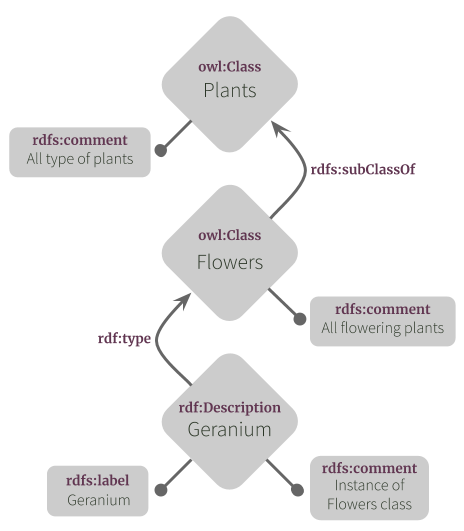
\includegraphics[scale=0.6]{img/owl-ontology-example.png}
\caption{An example of ontology defined using OWL and RDF Schema.}
\label{fig:owl-ontology-example}
\end{figure}

SPARQL is a query language for triplestores, a class of Database
Management Systems (DBMS) specialized in storing RDF databases. Such DBMS
often expose endpoints that can be used to query the database and obtain
results. Given the complexity of the data stored, the query language has
been designed to be as simple as possible, in example by allowing the use
of variables, whose definition is preceded by a question mark.

The syntax of SPARQL is heavily derived from SQL, with some
minor adaptations to be more suited for querying graph data. The
following is an example of query which selects all the labels
(human-readable description of a resource) of all the entities that
match the given resource type.

\begin{lstlisting}[
        language=sparql,
        frame=single,
    ]
    PREXIF plants:<http://example.org/plants/>

    SELECT ?name
    WHERE {
        ?subject rdf:type plants:flowers .
        ?subject rdfs:label ?name .
    }
\end{lstlisting}

\subsection{Knowledge Bases as knowledge repositories}

Even if the raise of the Semantic Web has suffered a slowdown in its growth
due to the complexity of its vision, many new projects were born from its
enabling technologies. Efforts have been put by profit and
non-profit organizations in trying to build complex knowledge repositories
starting from the knowledge already available in the Web. An example among all
is the DBpedia\footnote{\url{https://wiki.dbpedia.org/}} project, which
developed a structured knowledge base from the unstructured data available on
Wikipedia.
Another example is the
\emph{Google Knowledge Graph}\footnote{\url{https://blog.google/products/search/introducing-knowledge-graph-things-not/}},
which is used to enhance the Google search engine and virtual assistant
capabilities, allowing to retrieve punctual information about everything that
has been classified in its ontology and described in its knowledge base, or
the \emph{Open Academic Graph}\footnote{\url{https://www.openacademic.ai/oag/}},
a Scientific Knowledge Graph that contains, describes and links more then
three hundred million academic papers.

From an implementation perspective, knowledge bases can be created to
describe a specific domain by defining an ontology and a vocabulary for
such domain using OWL and RDF Schema, and then by describing the concepts
of such domain using the RDF Model and Syntax. The RDF document obtained
can then be stored in a triplestore and queryed using SPARQL. The biggest effort
when building knowledge bases is to have a correct understanding and prior
knowledge of the domain of interest, to avoid the risk of mischaracterizing
and misrepresenting concepts.

\begin{figure}[h]
    \centering
    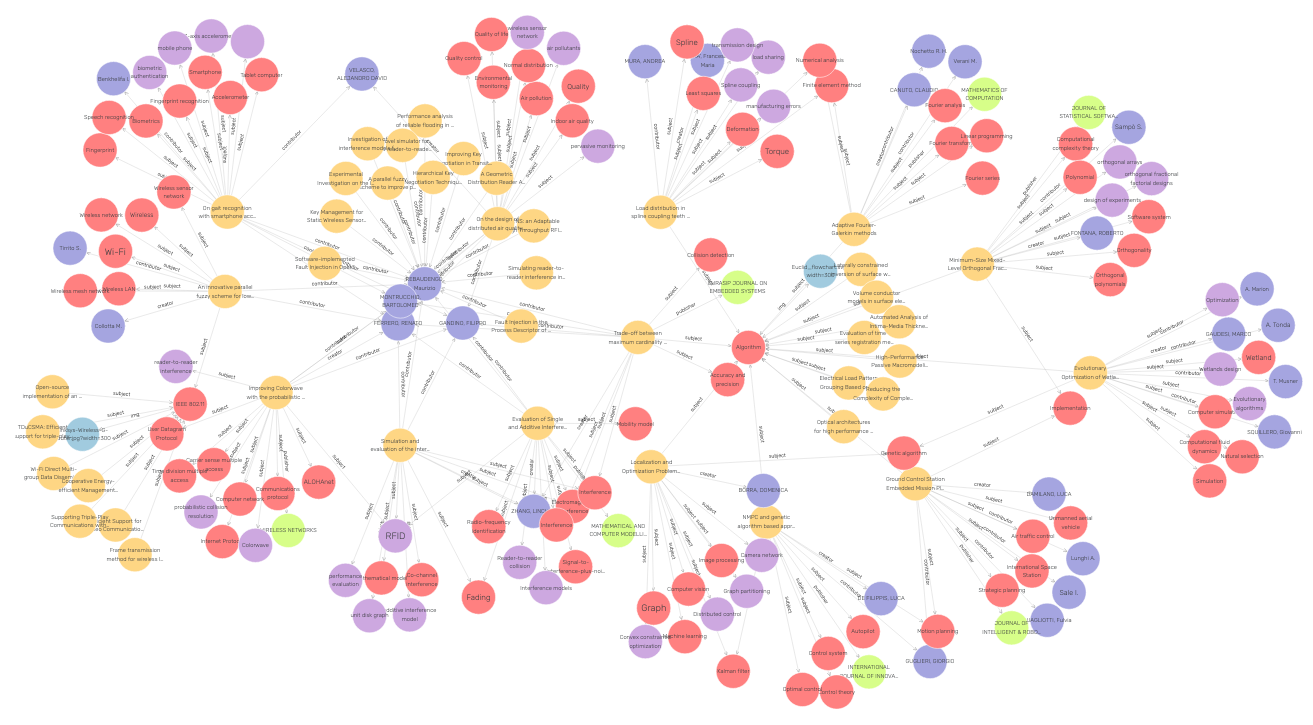
\includegraphics[scale=0.4]{img/geranium-knowledge-base-example.png}
    \caption{An extract of the Polito Knowledge Graph that will be introduced and
    described in the following chapters.}
    \label{fig:geranium-knowledge-base-example}
\end{figure}

If all the requirements and cautions are met, a well formed knowledge base may
prove to be a critical resource for an organization. It allows not only to
build new services upon it, but also to improve the existing knowledge inside
the organization by performing reasoning upon the available knowledge, thus
to discover implicit facts that can be derived from existing relationships.
Another field of applications is the development of Expert Systems, AI
software that emulates the behavior of a human decision-making process by
navigating the knowledge base and taking decisions like in a rule-based system.

Today's knowledge bases are commonly composed by tens of
thousands nodes and by hundreds of thousands of edges, such giant data
structures pose many challenges.
Not only storing and querying giant graphs requires the adoption of
specialized DBMS that are capable of efficiently store and query the RDF
input representation, but also doing analysis and gathering statistics from
such giant graphs requires the adoption of highly efficient algorithms in
order to retrieve the desired output in an acceptable time.

The availability of such a complex and informative data structure leads
to the opening of interesting scenarios, especially when thinking about
the latent information that can be extracted from it. In
fact, a knowledge base is a structured representation of the
human knowledge in a specific field, thus its comprehensiveness is restricted
by the human understanding.


\section{Learning on Graphs}

\subsection{Representation learning}

Machine learning (ML) algorithms are used to learn models from the
available data, with the final goal to obtain a set of parameters
that are fine-tuned to identify seen characteristics in the data
used for training. The obtained models can be used to
recognize unseen inputs by leveraging the knowledge embedded
in such parameters.
ML algorithms require the input data to be available in a
machine-understandable vector representation. An important task
in the ML field is the learning of such representations, task known
as representation learning.

Natural Language Processing (NLP) is one of the research branches that in
the past years has made a great use of machine learning algorithms both for
language recognition and for embedding words \emph{meaning} into words
\emph{vectors}.
One of the most successful algorithms when dealing with representation learning
of words is Word2Vec \cite{mikolov2013}, where the model obtained is trained to
learn a vector representation for each word in a vocabulary.
In Word2Vec, the concept of meaning of a word is related to the context in
which such word is frequently used, so two words are recognized as similar if
they're used in similar contexts, thus in the vector space of the learnt
representations words that have similar meaning have higher
cosine similarity\footnote{
    Cosine similarity is a heuristic method to measure the
    similarity between two vectors by computing the cosine of the angle between
    them:
    $similarity(A,B) = cos(\theta) = \frac{A \cdot B}{\Vert A \Vert \Vert B \Vert}$
}
with respect to dissimilar ones.
For instance, the cosine similarity between the word vectors of "Man" and "King"
is roughly the same as the one between the words "Woman" and "Queen", since such
words are used in similar contexts. This has open up new scenarios for
language recognition and processing, since it allowed to perform vector
operations on such words which brought interesting results, as can be seen
in Figure \ref{fig:word2vec}.

\begin{figure}[h]
    \centering
    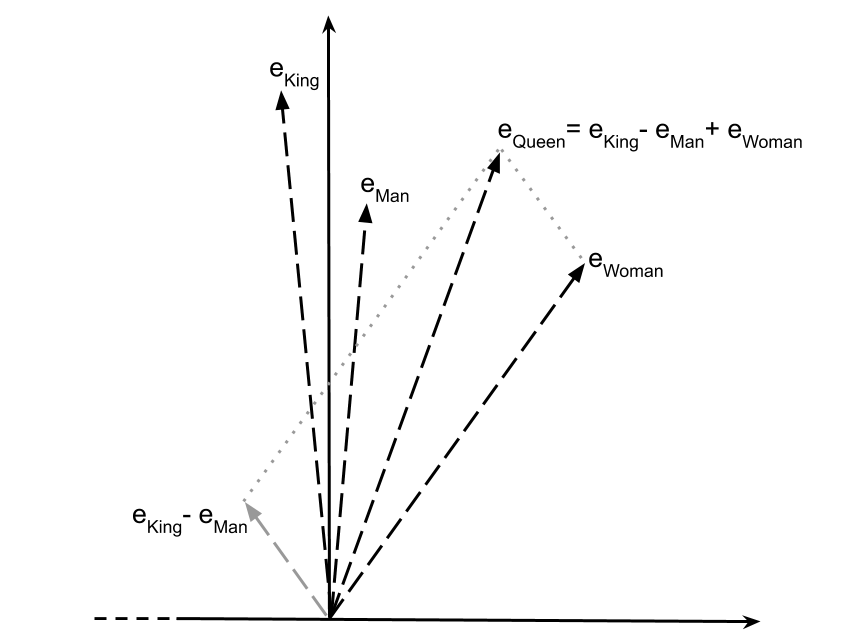
\includegraphics[scale=0.4]{img/word2vec.png}
    \caption{
        Word vectors allows to perform vector operations, the results
        obtained reflect the fact that Word2Vec is capable of embed the
        meaning of such words.
    }
    \label{fig:word2vec}
    \end{figure}

This idea of words characterized by the context in which they're used
can be generalized and applied to other fields of research, such as
the field of representation learning on graphs.

Graphs are composed by nodes and edges, and are used to describe complex
systems, such as social networks or the interactions in a molecular biology
system. To apply machine learning algorithms to such data structures
vector representations of nodes and edges are needed in order
to be able to learn from the available data and predict new facts.
Such vector representations are often referred to as \emph{embeddings} because
they should embed the characteristics of the graph nodes, so that similar nodes
have similar embeddings. In example, in a scholarly knowledge base publications
with same authors and similar subjects should have similar embeddings.

Early approaches required these representations to be learned from feature
vectors that where handcrafted, task that required not
only a relevant amount of effort, but also a deep understanding of the domain
of interest. This has long been one of the main obstacles when dealing with
representation learning tasks, since who has knowledge of the domain and who
has to engineer the features were unlikely the same individual.


\subsection{Deep Learning on graphs}

In the latest years a big shift towards deep architectures has been made
in machine learning, mainly thanks to the development of highly
parallelized architectures that are able to efficiently compute
at the hardware level vector and matrix multiplications, operations that
are at the basis of any machine learning task.
Deep Learning (DL) algorithms are able to extract relevant features from
raw data by applying simple mathematical operations, such as convolution, to
the input data.
An example of one of the most successful applications of DL is in
image recognition, where matrix representations of images are
convolved with self-trained filters that are able to
extract the relevant features needed to recognize patterns present
in the input images.

Deep learning techniques have proven to perform well also in the field of
representation learning for graph data.
As can be seen in figure \ref{fig:pixels-as-graph}, a digital image
is composed by pixels which can be thought of as nodes in a graph, where
each pixel is connected by an edge to its immediate neighbors. This suggests
that the techniques used when dealing with images can be adapted, with
some major changes, to the field of representation learning on graphs, but
also in other fields of research, such as learning on manifolds.

\begin{figure}[h]
    \centering
    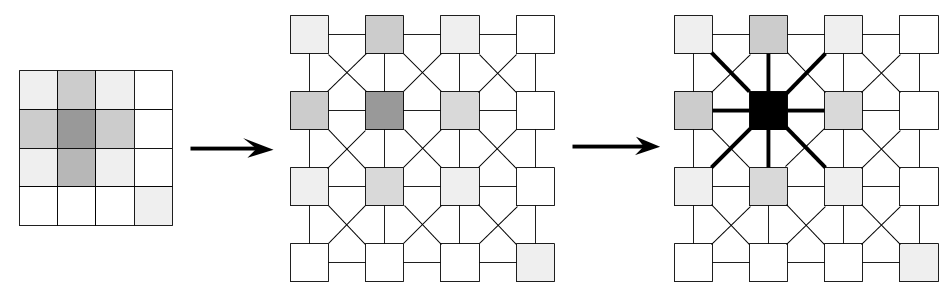
\includegraphics[scale=0.4]{img/pixels-as-graph.png}
    \caption{A digital image can be thought of as a graph.}
    \label{fig:pixels-as-graph}
\end{figure}

The issue of working with graph data is that commonly graphs
are built to describe complex systems, such as the knowledge of a
domain or field for knowledge graphs, and thus are composed of
a fairly high amount of nodes and edges. The matrices used to
store the graph structure can thus explode in dimensionality, becoming
impractical as input data. Moreover, graphs are not
regular structures with a given shape and size, such a matrix of pixels
for images, but they live in an irregular domain which led to highly
irregular structures.
The first issue can be solved by randomly sampling the graph at each
training epoch, the immediate drawback being that more than one epoch
is required to train over all nodes. The second issue can instead be
solved by adapting known algorithms to work on irregular domains.
One of the possible approaches, which has proven to work well, is
the one based on convolutions.

Graph Convolutional Networks (GCNs) \cite{kipf2016} are a class of
semi-supervised deep learning algorithms for graphs which are based on the
same convolution and backpropagation operations as the well known
Convolutional Neural Networks (CNNs) used for feature learning on
images.
The main difference between CNNs and GCNs is in how the convolution is
performed, instead the backpropagation phase is the same as the one
used to update the parameters of CNNs, with a task-specific loss function.
In a CNN the input matrix of each network layer, which is the pixel matrix
of the input image for the first layer, is convolved with a convolutional
filter, whose parameters are then updated during the backpropagation phase.

GCNs works similarly by convolving at the l-th layer
of the network the feature vector of each node with the feature
vectors of its l-nearest neighbors, this is done by applying the following
transformation:

\begin{equation} \label{gcn1}
H^{l+1}=\sigma(\tilde{D}^{-1/2}\tilde{A}\tilde{D}^{-1/2}H^lW^l)
\end{equation}

Where $H^{l}$ is the output of the previous layer or, for the input layer, the
node features matrix where each row is commonly initialized
as a one-hot encoded feature vector. $\tilde{A}$ is the adjacency matrix
of the graph summed with the identity matrix to add self loops of nodes,
$\tilde{D}$ is the node degree matrix of $\tilde{A}$ and is used to
normalize it, $W^l$ is the weight matrix of the layer, that is shared
among all nodes for each layer, just like the convolutional filter in a CNN,
and $\sigma()$ is a non linear activation function, for example $ReLU$.

The forward rule to update the embedding of a single node at each
layer of the network is the following:

\begin{equation} \label{gcn2}
    h^{(l+1)}_{i}=\sigma(\sum_{j\in\eta_{i}} \frac{1}{c_{i,j}}h_j^{(l)}W^{{(l)}})
\end{equation}

Setting aside the normalization costant $c_{ij}$ which is obtained from the
multiplication between the adjancency and degree matrices, at each layer the
updated feature vector of the node $i$ is obtained by summing over all the
nodes in its neighborhood the result of the multiplication between the
neighbors feature vectors and the weight matrix of the layer.
A consequences of applying this rule to all nodes is that at the l-th layer
the feature vectors of nodes that are at a $l$ hop distance from the node $i$
will be embedded in its feature vector, because the feature vectors of such
nodes were embedded, at the previous layer, by the immediate neighbors of
node $i$, which are now passing the information of their surrounding to it.
So the amount of layers of the network is a parameter that controls how much
information from furthest nodes has to be collected by each node embedding.

\begin{figure}[h]
    \centering
    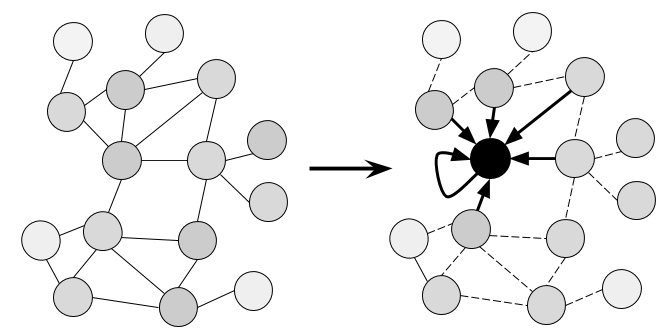
\includegraphics[scale=0.4]{img/gcn.png}
    \caption{First layer of a GCN updating a node feature vector by embedding
        the features of adjacent nodes.}
    \label{fig:gcn}
\end{figure}

As a result of the propagation step each node embedding will be characterized by
its context, just like it happens in Word2Vec, but in a non-Euclidean domain.
So for example, in a social graph where each person is characterized by its
friends, interests, places visited and so on, two people will have similar
embeddings if they are connected to similar nodes.

The node embeddings obtained by applying a GCN or one of its variants can
then be used to perform some learning task on the graph, two examples are
the classification of unseen nodes or the link prediction of non-existent
edges. The last example is one of the most interesting tasks because it empowers
most of the recommendation systems available in the industry.


\subsection{Link prediction on Knowledge Graphs}
\label{subsec:linkprediction}

Predicting new facts is one of the most common task in the field
of knowledge graph completion. The goal of such task is to evaluate if unseen
good candidates to be included in the knowledge base.
Link prediction requires two main step:

\begin{enumerate}
    \item Train an encoder model
    that is able to embed the node features and produce meaningful embeddings.
    \item Apply a factorization model that is able to score the unseen
    triples under evaluation.
\end{enumerate}

Deep learning techniques such as GCN can be exploited to obtain meaningful
node embeddings, but fall short when dealing with graphs where
nodes are connected by different relations (multi-relational graphs).
In fact, if we use a single layer GCN to obtain the embeddings of two nodes
that share the same neighborhood, but are connected to the neighbors via
different relations, we'll obtain almost the same embeddings, even if it's
clear that they do not share the same characteristics. For example in a
producer-consumer framework one node could be the producer while the other
the consumer, having both a common neighborhood of nodes
which are produced by the former and consumed by the latter.
If a GCN is used, the embeddings obtained would be very similar, even if
the two nodes clearly don't have the same role and don't belong to the
same class.

To overcome this limitation, changes to the basic GCN architecture have been
proposed, so to obtain models that works well when applied to multi-relational
graphs.
\newline

Relational Graph Convolutional Networks \cite{schlichtkrull2018} (R-GCNs) are an
extension of GCNs that are focused on modeling multi-relational graphs composed
by directed edges, and thus are particularly capable of embedding both
nodes and relations of a knowledge graph.
R-GCNs can be used for both link prediction and node classification tasks.

At an high level the R-GCN architecture can be seen as a special case of
the \emph{message passing framework} \cite{gilmer2017}, which groups together
under a common scheme most of the existing neural models for graph data.
The framework defines two major phases: a per-edge message computation and a
per-node message reduction.
In the first phase a function or linear transformation is applied to each edge
to obtain an edge specific message.
Then, in the reduce phase, the embedding of each node is updated by aggregating
together all the messages of the incoming edges.

This two phases can be grouped together through by the following equation:

\begin{equation}
    h_i^{(l+1)} = \sigma \left(
            \sum_{m\in{\CMcal{M}_i}} g_m(h_i^{(l)}, h_j^{(l)})
        \right)
\end{equation}

Where $\CMcal{M}_i$ is the set of incoming messages for node $i$ and
$g_m$ is a message specific transformation.
\newline

The idea behind R-GCN is to have different set of parameters
for different relations.
At each step inside the network, the feature vector of a node is updated by
convolving its first neighbors features with a convolutional filter that is
different based on the kind of relation that connects the nodes.
The forward
rule to update the embedding of a node at the \emph{l} layer is the following:

\begin{equation}
    h^{(l+1)}_{i} = \sigma \left(
        W_0^{(l)}h_i^{(l)} + \sum_{r\in\CMcal{R}}\sum_{j\in\CMcal{N}_i^r}
        \frac{1}{c_{i,r}} W_r^{(l)} h_j^{(l)}
    \right)
\end{equation}

Where $h_i$ is the embedding (or, for the first layer, the input feature
vector) of the node \emph{i}, $W_0$ is the learnt kernel for the
relation between the node and itself (called self loop), $\CMcal{N}_i^r$ is the
set of indices of the neighbors of node \emph{i} under the relation
$r\in\CMcal{R}$, with $\CMcal{R}$ being the set of all the relations present in
the graph. $W_r$ is the learnt kernel for the relation $r$.
As for the GCN architecture, $\sigma$ is a non linear activation function
and $c_{i,j}$ is a normalization constant, commonly initialized
to $|\CMcal{N}_i^r|$.

From a message passing framework perspective, the message function (per-edge
transformation) is equal to the linear transformation $W_rh_j$, and the reduce
function (per-node transformation) is just the sum of
all the messages computed for the incoming edges of each node.

As can be seen the update rule looks similar to the one for GCNs (\ref{gcn2}),
with the major difference that in the case of a R-GCN the parameters used to
convolve the
feature vectors of neighboring nodes are relation specific, this means that
the kind of relation that connect the node to its neighbors has an important
role in determining the node embedding.

\begin{figure}[h]
    \centering
    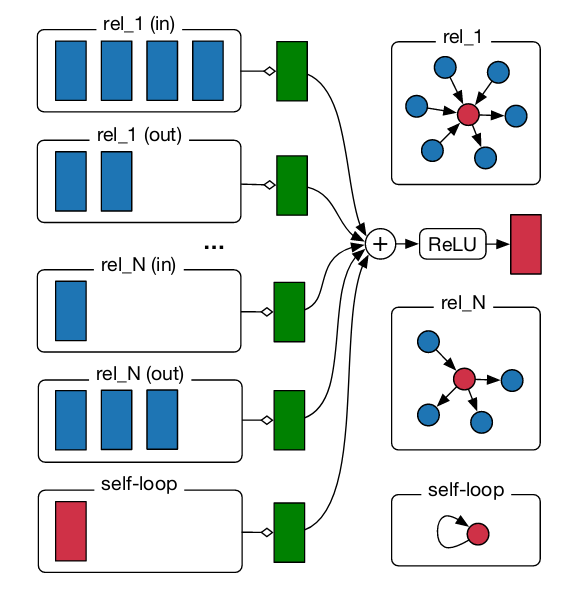
\includegraphics[scale=0.5]{img/rgcn-encoder.png}
    \caption{R-GCN encoder model. Image taken from \cite{schlichtkrull2018}.}
    \label{fig:rgcn-encoder}
\end{figure}

Some form of regularization is required in order to avoid overfitting on rare
relations, thus to obtain a more generalized model, and also to avoid
the rapid growth in the number of parameters of the network for
highly multi-relational graphs. One of the solutions proposed by the original
paper \cite{schlichtkrull2018} is to decompose each relation filter $W_r$
using basis decomposition:

\begin{equation}
    W_r^{(l)} = \sum_{b=1}^B a_{r,b}^{(l)} V_b^{(l)}
\end{equation}

This allows to store only the relation-specific coefficients and the basis,
which will be shared by all the relations.

The model obtained by training an R-GCN can then be used to build an encoder
that given as input a graph, gives as output the embeddings of all nodes and
the relations parameters. Then a factorization method can be used to
evaluate unseen facts inside the graph, exploiting the resulting embeddings.
Such methods are used as scoring functions in order to obtain, starting from
the entities embeddings, a real value that can be used to score the unseen
triples under evaluation.
\newline

DistMult \cite{yang2014} is one of the most common and simple factorization
methods used to score unseen triples. Given as input the embeddings of the
source node and destination node, and the relation parameter vector
transformed into a diagonal matrix $R_r\in\mathbb{R}^{d \times d}$, it computes
an associated real valued score:

\begin{equation}
    f(s,r,o) = e_s^T R_r e_o
\end{equation}

The score obtained by applying such function can then be used to evaluate
wether the triple $(s,r,o)$ is a good candidate to be added to the graph, an
high score is to be interpreted as a high confidence of the model
in the fact that the triple should belong to the knowledge graph.



\chapter{Approach and methodology}

This chapter introduces the software architecture developed to build, enhance
and visualize the Polito Knowledge Graph (PKG), an academic RDF graph
built to organize in a structured and semantically coherent way the publications
produced by the researchers of the Polytechnic University of Turin. The graph
also includes publication-related entities, such as authors, journals,
and field of study.

The architecture, which is showed in Figure \ref{fig:pipeline}, is structured
as a pipeline composed of three main building blocks:

\begin{enumerate}
    \item The \emph{graph builder}, which creates a first version of the
    RDF graph.
    \item The \emph{graph enhancer}, which implements ML techniques to predict
    unseen facts. Such facts can then be added to the graph to improve its
    completeness.
    \item The \emph{viewer component}, a web application that allows to query
    and visualize the graph data.
\end{enumerate}

At an higher level the components of the architecture can be divided in
producers and consumers, where the former produces the graph data, and the
latter consumes the data produced.
The \emph{builder} act as producer taking as input the IRIS data
and producing a set of RDF statements that together composes the
Polito Knowledge Graph.
The \emph{enhancer} act as both a producer and a consumer, given that it
takes as input the PKG and use it to predict unseen facts that can be
later added to it as RDF statements.
The \emph{viewer} consumes the graph by storing it a triplestore and exposing
a public web interface for querying and visualizing the data.


\begin{figure}[h]
    \centering
    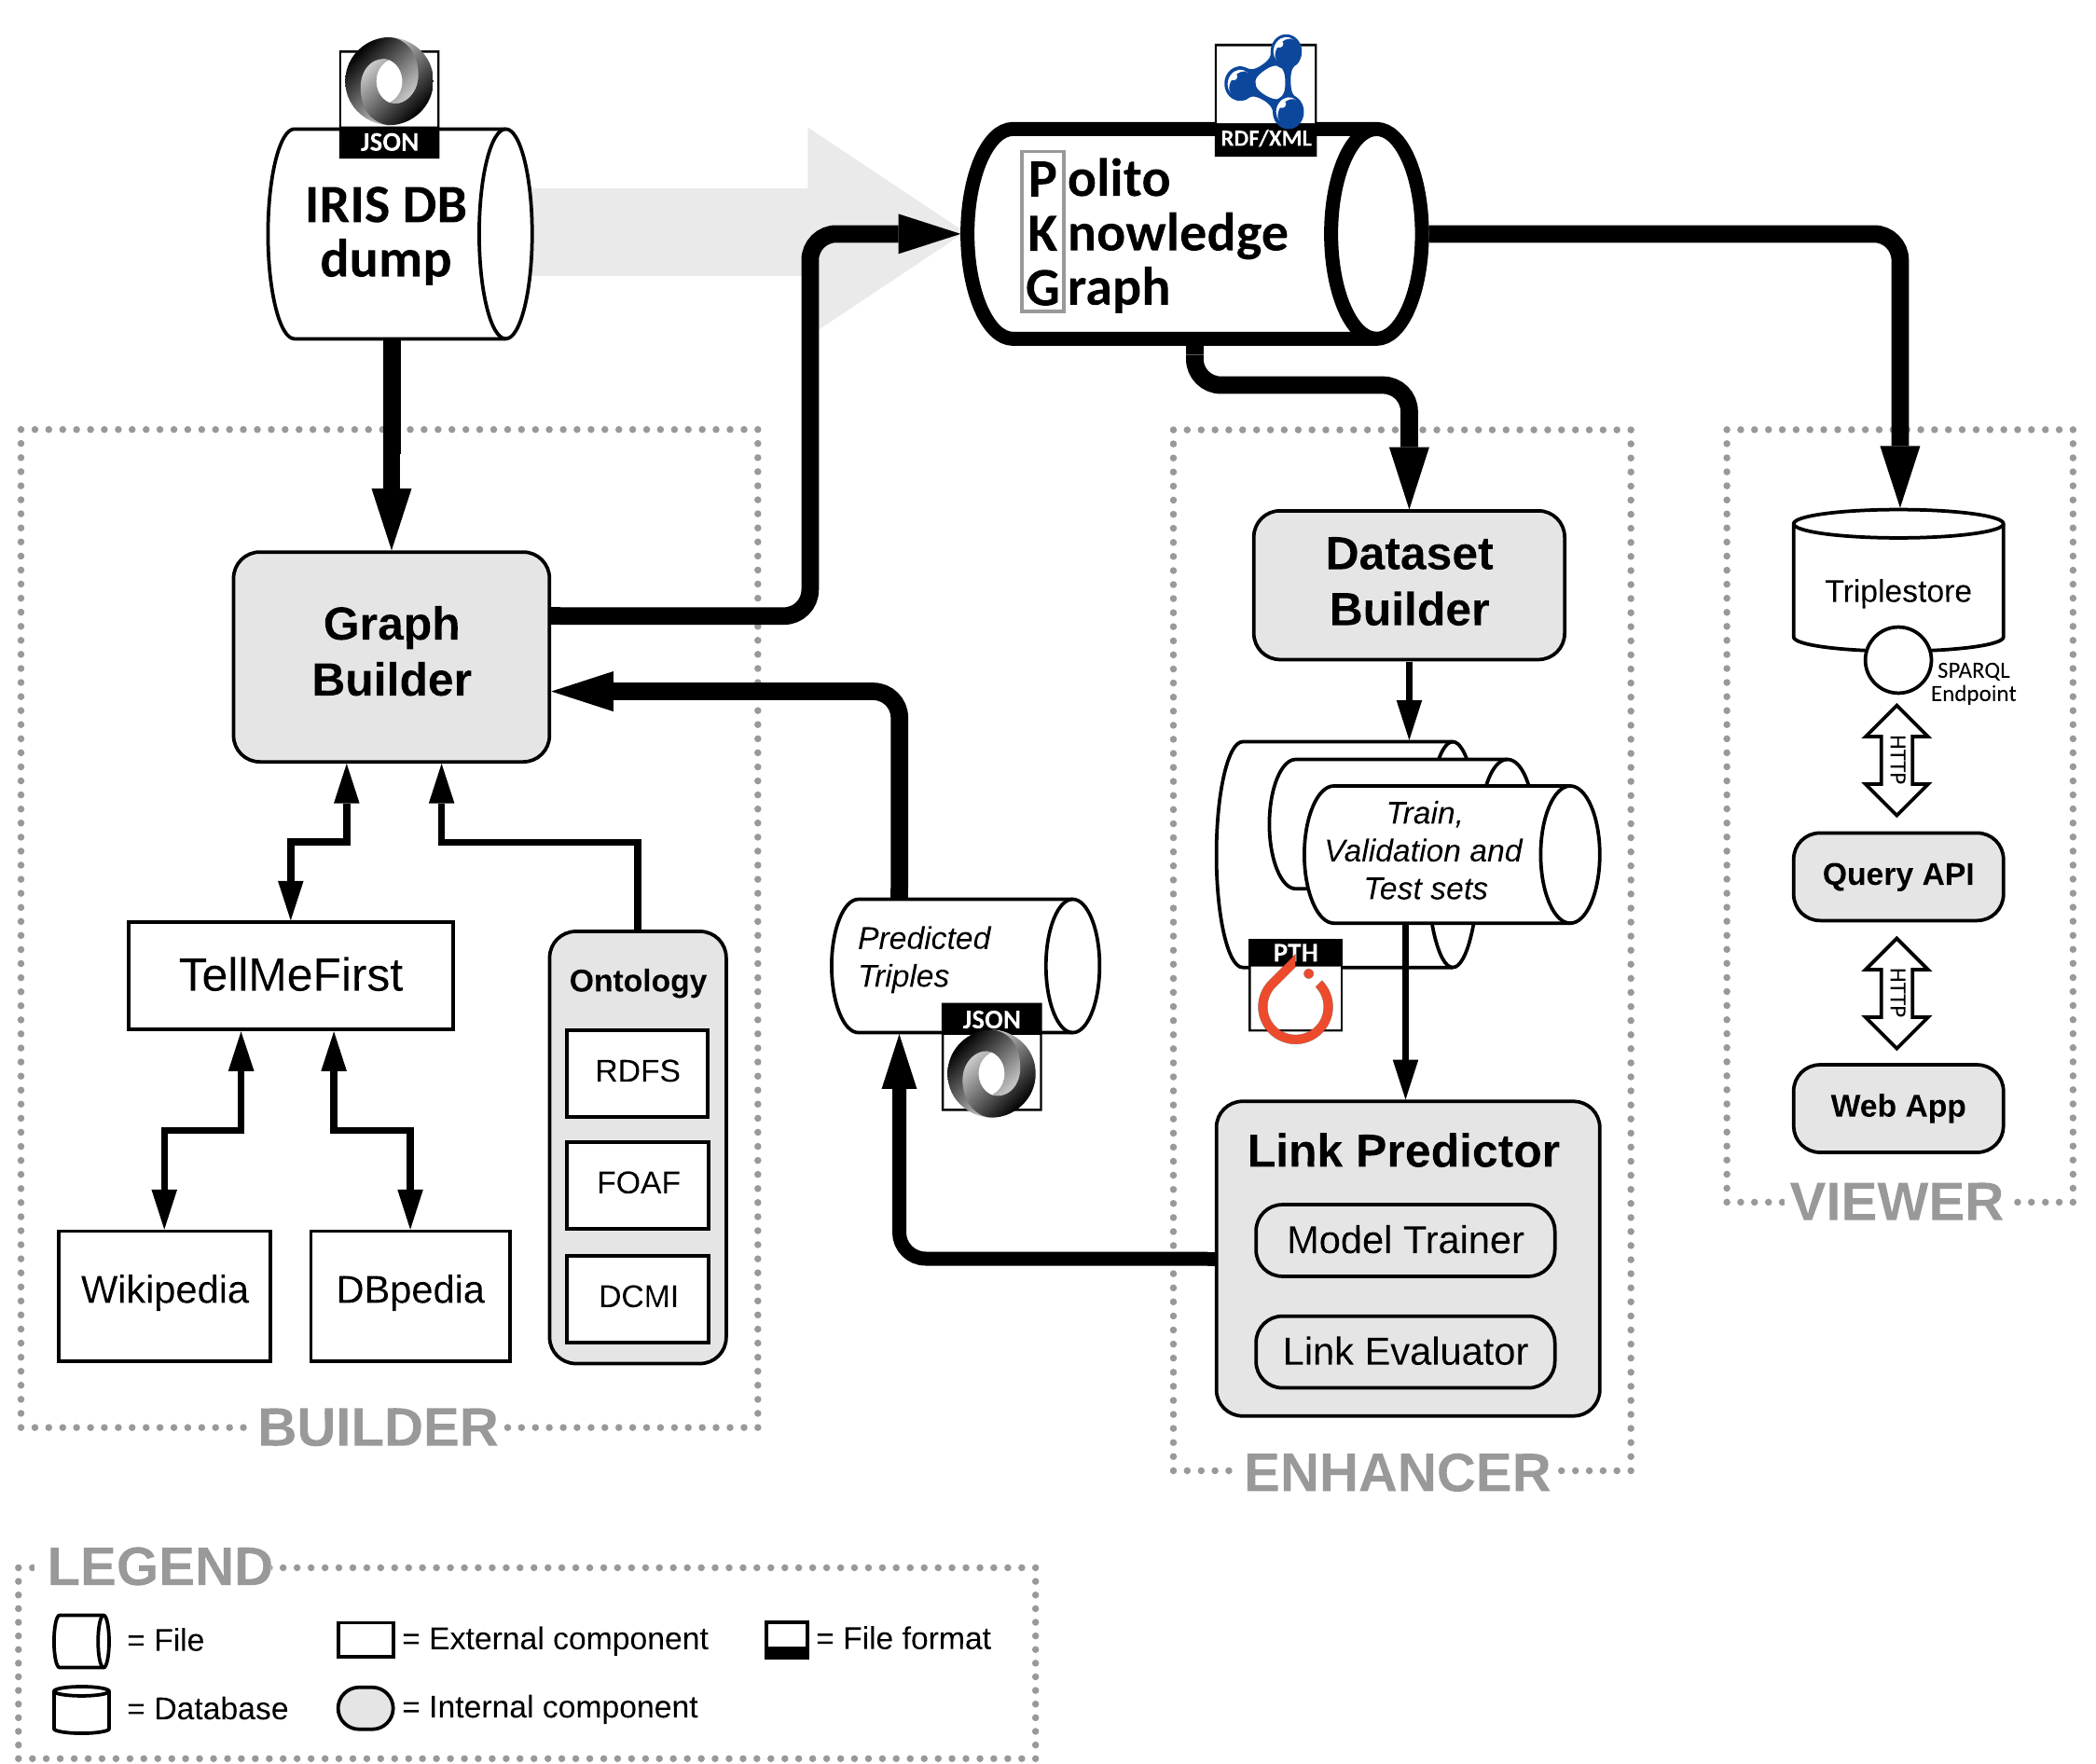
\includegraphics[scale=0.8]{img/pipeline.png}
    \caption{Pipelined software architecture developed to build,
    enhance and visualize the Polito Knowledge Graph.}
    \label{fig:pipeline}
\end{figure}


\section{Builder architecture}

The graph builder input is a database dump of
IRIS\footnote{\url{https://iris.polito.it/}}, which is the platform
used by the Polytechnic University of Turin to store and share all the
publications made by its researchers. The dump is a JSON file that contains
all the information available for every scientific paper published in a period
of five years that goes from 2013 to 2017.

The builder role is to translate all the information contained in the dump in a
set of semantically coherent RDF triples. To do so, an ontology that
describes the domain of the IRIS scholarly data has been defined.

The builder uses as reference the defined ontology to analyze each record in
the JSON dump, and build facts as RDF triples by matching the information
contained in the record with the concepts defined by the ontology.
For example, given that a publication may have more then one contributor, the
ontology differentiates the principal author from the contributors by using two
different statements to tie the corresponding entities to the publication.

One of the fields of the publication record is the abstract. We wanted to
tie each publication to its main topics, to do so we used the abstract
as input text for TellMeFirst \cite{rocha2015}, a tool for the automatic
extraction of semantic keywords from texts. This keywords, to which from now
on we'll refer to as \emph{topics}, are retrieved from the DBpedia taxonomy
and are uniquely identified by their corresponding URI.
Exploiting TellMeFirst we are able to automatically tie each publication to
its relevant topics, by adding the corresponding RDF statements to the graph.
This has as consequence that the topics are added to the graph, and being
uniquely identified, all the publications that share a topic are
bounded to the same topic entity.

The result of this process is a semantically coherent description of all the
publications linked with their authors, contributors and relevant topics.
The set of all this RDF statements composes the Polito Knowledge Graph.


\section{Enhancer architecture}

Once the RDF graph has been built, it could be used as input for the enhancer
module, whose main role is to leverage ML techniques to predict new triples
that could be good candidates to be included in the graph.

The enhancer architecture is splitted in three main components:

\begin{enumerate}
    \item The dataset builder.
    \item The model trainer.
    \item The link evaluator.
\end{enumerate}

The first component is in charge of translating the RDF graph into a usable
dataset for the model trainer, given that RDF statements cannot be used as
input data for the link prediction algorithm.
The dataset will then be splitted into three disjoint sets: one for training,
one for validation and one for testing.
The model trainer uses this three sets to train a link predictor. The train
set is used to train the model at each epoch, while the validation set
is used to evaluate which model parameters to keep, identifying the best epoch.
The test set is used to evaluate the accuracy of the model loaded with the best
epoch parameters upon unseen triples.

Once the model has been trained, it can be used to predict unseen facts.
The link evaluator loads the best model found during the training phase and
uses it to evaluate unseen facts.
The evaluator creates an set of unseen RDF triples and produces a score for
each of them. Only the triples that obtain an high score (and so an high
probability to be true facts) and are correct in domain and range with respect
to the ontology are kept.
The predicted triples are then saved as RDF statements and could be added
to the RDF graph, obtaining an enhanced knowledge graph completed with
latent information automatically extracted.

\section{Viewer architecture}

The last component of the architecture is the viewer, which is composed of a
triplestore, an API layer, and a front end web interface.

The triplestore is a specialized DBMS for storing and retrieving RDF
statements.
It stores an online copy of the Polito Knowledge Graph and expose a
SPARQL endpoint that allows to query the graph itself.

The API layer exposes a REST API that allows to retrieve the information
contained in the graph without the need of SPARQL queries. It accept HTTP
requests with URL-encoded parameters and proceeds to query the SPARQL endpoint
of the triplestore by matching the parameters upon some predefined queries.
Then it translates the response obtained from the triplestore in a JSON,
which is sended back to the requesting client, which is typically the front end.

The front end is a responsive web application that act as the entry point for
the user, mimicking the functionalities of a modern search engine. It allows
to query and visualize the data contained in the graph by
performing HTTP requests to the API layer and displaying the results received
in a structured and comprehensible way.


\chapter{Related work}

% Open Academic Graph
In the past years there has been a growing interest in scientific
knowledge graphs, both by academic institutions and by private organizations.
An example is the Open Academic
Graph\footnote{\url{https://www.openacademic.ai/oag/}} (OAC), an academic
knowledge graph built by unifying two of the largest
scientific KG available, the Microsoft Academic
Graph\footnote{\url{https://academic.microsoft.com/}}
and AMiner\footnote{\url{https://www.aminer.cn/}}.
It has been publicly released to allow
the study of citation networks, papers content and more.
The first version of the graph, released in 2017, has been
built by merging together the aforementioned graphs and by linking the
matching publications, obtaining a graph that is composed by more then three
hundred million publications. In the first version the only type of entity
in the graph was the publication: authors, journals, and all the other
publications information were added as attributes, and not as entities.

In January 2019 the second version of the OAC has been released, adding even
more publications to the graph. However, the biggest change of this new
version is the addition of authors and venues as graph entities,
instead of being simple publications attributes.

However, the OAC doesn't contain the publications topics as graph
entities, but as author keywords, thus being prone to the same limitations of
IRIS: the keywords are the ones chosen by the authors and are not
referencing to semantic concepts, being simple character strings.
\newline

% wiser
Regarding the development of tools similar to the Polito Knowledge Graph
by other academic institutions, an example of employment of knowledge graphs
and natural language processing techniques is Wiser\cite{cifariello2019}, an
expertise search tool developed by the University of Pisa and publicly released
at the beginning of 2019.
The KG of Wiser is composed of approximately 1'500 authors, 65'000 publications
and 35'000 topics. This numbers will be compared to the one of the Polito
Knowledge Graph in the following chapter.
The main function of Wiser is to allow the search of expertise in a given
research field.
The system has proven to be particularly effective, representing a strategic
tool and being actively used by the university technological transfer office.
\newline

% CSO Classifier and Computer Science Ontology
As saw in the previous chapter, one of the main components of the PKG
pipeline is TellMeFirst, tool used to automatically extract the topics of
interest from the publications abstracts. By automatically extracting the
topics, TMF allows to add them as entities in the Polito Knowledge Graph,
so that each publication is directly linked to its main topics, and each topic
is linked to all the publications of which it is a subject (reverse relation).

Other tools that are able to extract the subjects of a publication exists, an
example is the CSO Classifier \cite{salatino2019}. This tool is able to
automatically classify a research paper according to the Computer Science
Ontology\footnote{\url{https://cso.kmi.open.ac.uk/home}} (CSO), an automatically
generated ontology of research topics in computer science.
The fact that the CSO Classifier relies on a predefined ontology has some
disadvantages with respect to TellMeFirst, the biggest being the fact that the
Computer Science Ontology is restricted to the computer science field only,
while TMF, using DBpedia as its source of knowledge, is able to extract
topics (and so classify a research paper) regarding every field of research.
However, the approach of CSO Classifier has also its advantages: being the
ontology more restricted, the classification could be more accurate, and the
structure of the ontology itself may be tailorized for such classification task.

% R-GCN
Regarding the prediction of unseen links inside the graph, to the best of our
knowledge we are the first to employ a Relational GCN for the completion task
of a scholarly knowledge graph.



\chapter{Development and implementation}

In this chapter we will describe how we developed and implemented the
architecture behind the Polito Knowledge Graph, particularly focusing
on the components in charge of the graph creation and enhancement, whose
architecture has been introduced in the previous chapter.

We will firstly introduce a detailed description of the input data used to
create the graph. We will also describe the ontologies used to shape the
knowledge of the scholarly domain and the resulting graph schema, obtained
by shaping the available IRIS data using such ontologies.
Then, we will look at the implementation of the graph builder, the component
responsible for the actual creation of the RDF graph.

In the second part of the chapter we will focus on the implementation of the
link predictor component. We will describe how the RDF graph is used to
generate a usable dataset for the training of a machine learning model, how we
trained such model and which hyperparameters we used. We will also discuss
the metrics used to evaluate the model, and how we employed the trained
model to obtain meaningful predictions about missing links inside the graph.


\section{Building the Polito Knowledge Graph}

As already mentioned when introducing the pipeline, the input data used to
build the PKG is a dump of the IRIS database which contains the
scientific papers published by the researchers of the Polytechnic University
of Turin from the beginning of 2013 to the end of 2017.
The dump is a JSON file composed of 23'268 records, where each record contains
the metadata about a singular scientific publication.
Many of the metadata present are generated by the IRIS platform itself in
order to manage its internal processes of acceptance and update of the
publication status. We have discarded such metadata, since they do not
represent significant information for the characterization of the publication.

We selected the following metadata for building the graph, being the ones that
truly represent semantic information about a publication:

\begin{enumerate}
    \item The publication identifier.
    \item The title.
    \item The abstract.
    \item The author name, surname and identifier.
    \item The contributors name, surname, and identifier (if present).
    \item The date of publication.
    \item The journal title and ISSN (if present).
    \item The keywords inserted by the authors.
\end{enumerate}

The publication identifier is a unique number associated by IRIS to each
scientific paper. Also the authors and the contributors are uniquely identified
by an alphanumeric identifier, however, only the researchers of the Polytechnic
University of Turin have such identifier assigned. External researchers that
may be contributors or co-authors of the publication have only their name
and surname listed.
If the information about the journal is present, then the journal ISSN is
used as identifier.
The title, the abstract, the names, surnames and the keywords are simple
character strings, while the date is in "dd-mm-yyyy" format.

As already discussed in previous chapters, the keywords inserted by the authors
cannot be treated as semantic concepts. We wanted to solve this issue, in order
to have all the publications that refer to a specific topic linked to a
same semantically unambiguous graph entity that uniquely represents such topic.
To do so, we employed TellMeFirst (TMF), a tool for the automatic extraction of
semantic keywords that relies on the DBpedia ontology and knowledge graph as
its source of knowledge.
In the following sections we will describe how we developed the graph builder
and how the use of TMF allowed us to add the semantic concepts extracted from
the publications abstracts as graph entities of the Polito Knowledge Graph.


\subsection{PKG ontology and schema}

We defined the PKG ontology as composed of five different classes:
the \emph{Publication}, the \emph{Author}, the \emph{Journal}, the
\emph{AuthorKeyword} and the \emph{TMFResource}.

In order to build a knowledge graph, the instances of such classes must be
linked together by means of semantic relations, called predicates.
To do so, we employed some predicates already defined by the FOAF and the
DCMI ontologies, together with some terms defined by the RDFS standard.
The graph structure obtained is represented by the schema in
Figure \ref{fig:schema}, where the classes, the attributes of such classes and
the predicates that link them together are showed.

\begin{figure}[h]
    \centering
    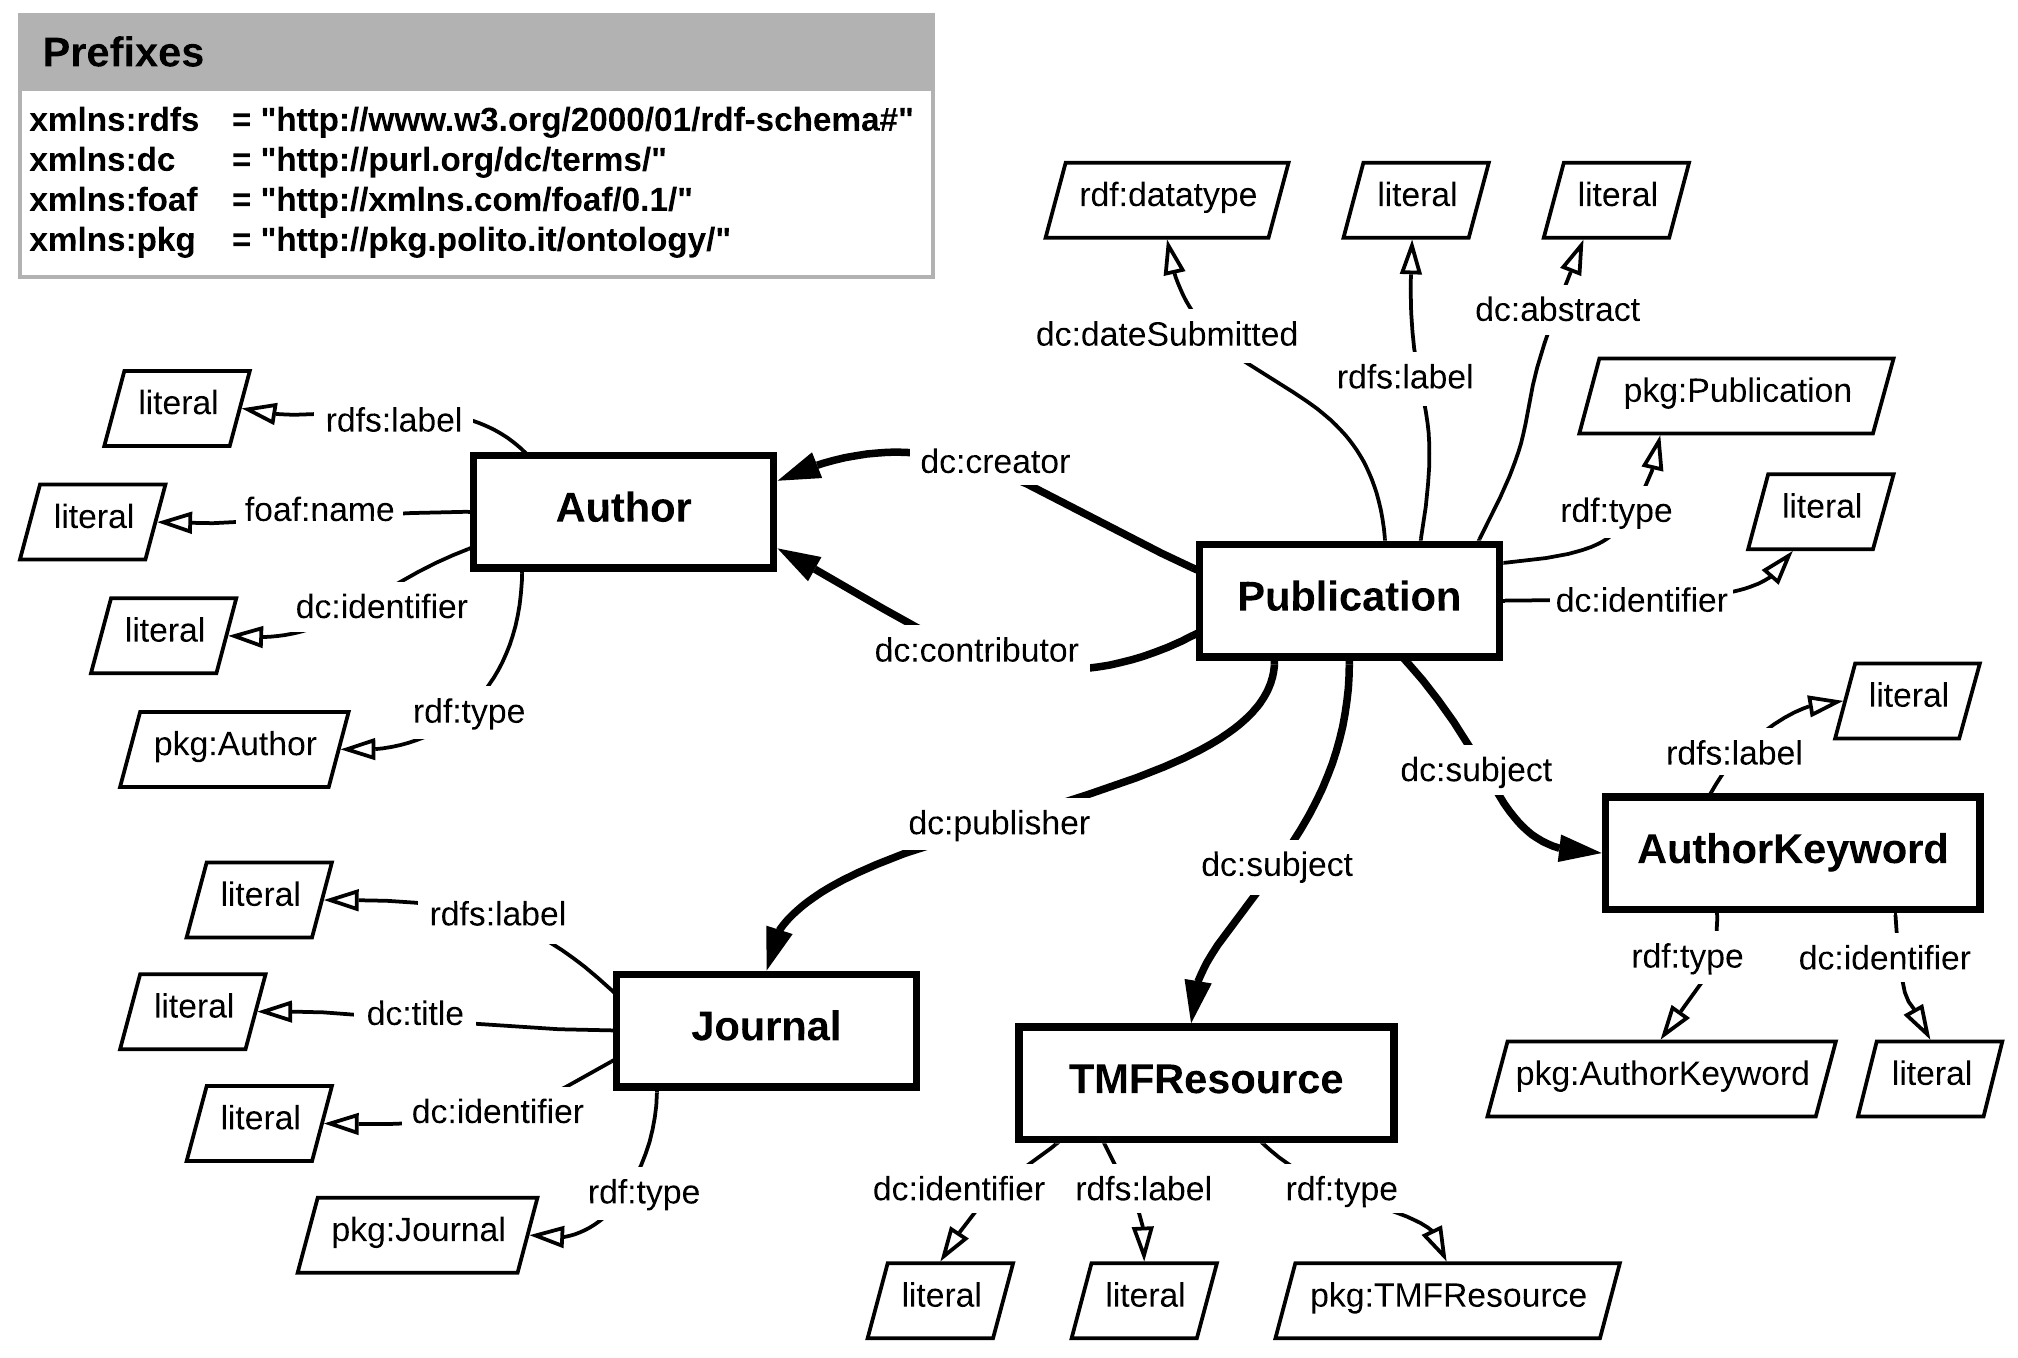
\includegraphics[scale=0.20]{img/schema.png}
    \caption{Schema of the Polito Knowledge Graph. The ontologies used to
    define the structure are showed in the prefixes table.}
    \label{fig:schema}
\end{figure}

As can be saw from the schema of Figure \ref{fig:schema}, the \emph{Publication}
class is linked to the author class by means of two relations both defined by
the DCMI ontology: \emph{dc:creator} and \emph{dc:contributor}.
We decided to only differentiate the first author (creator) from
the others (contributors) due to the inability to discriminate which are the
co-authors and which are the collaborators.

The \emph{AuthorKeyword} class refers to the keywords inserted by the authors,
they're kept for the sake of completion with respect to the metadata available
in the dump, but they do not represent any semantic information.

Instead, the \emph{TMFResource} class is used to instantiate the DBpedia
resources that are extracted by TMF from the publication abstract. Being
uniquely identified by their DBpedia URI, each instance will be unique, and so
if more publications shares the same extracted subjects, they will be linked
by the \emph{dc:subject} relation to the same instance of the corresponding
\emph{TMFResource}. An example is showed in Figure
\ref{fig:subject-knowledge-base}, where are showed all the publications that
are linked to the TMFResource of the topic \emph{Knowledge Base}.

\begin{figure}[h]
    \centering
    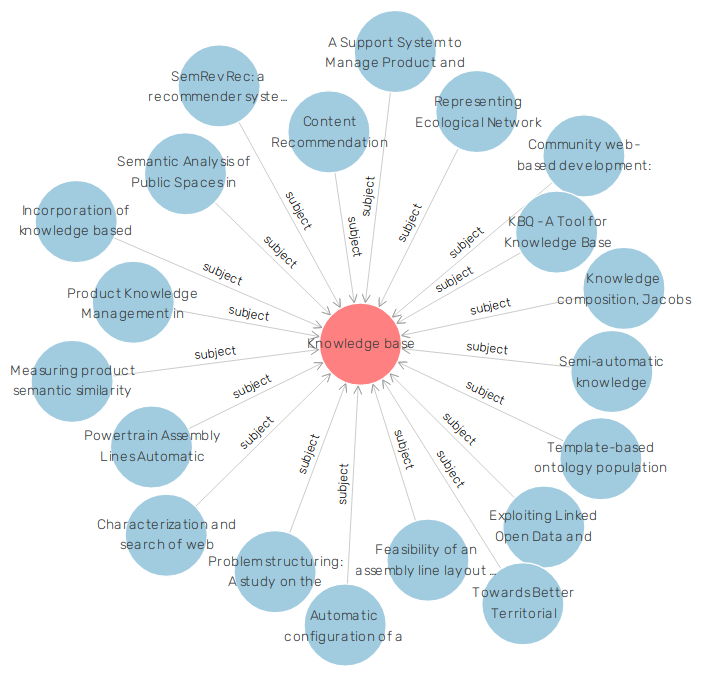
\includegraphics[scale=0.40]{img/subject_knowledge_base.png}
    \caption{Visualization of the result obtained from
        the Polito Knowledge Graph when running a SPARQL query that returns
        all the publications that have \emph{Knowledge Base}
        as subject.}
    \label{fig:subject-knowledge-base}
\end{figure}



\subsection{The graph builder}

We implemented the graph builder as a Python command-line script that uses
the \emph{rdflib}\footnote{\url{https://github.com/RDFLib/rdflib}} library
to create and manage an in-memory RDF representation of the graph that could be
then serialized and saved as an XML file.
The script takes as arguments the path of the JSON dump of IRIS, together
with some options that allows to trigger specific functionalities of the
script, such as:

\begin{enumerate}
    \item The update of an already existing RDF graph, this allows to add new
        RDF triples without the need of rebuilding the graph from scratch.
    \item The number of topics that must be extracted from each abstract by
        TellMeFirst, the default value is seven.
    \item The addition of the topics images, which are scraped from DBpedia and
        added as attributes of the \emph{TMFResource} instances.
\end{enumerate}

The script firstly declares the namespaces and the ontology used to define the
RDF representation of the entities and the relation inside the graph as written
in the previous section, then parses the arguments and options received and
execute the corresponding activities.

If the creation of a new graph is requested, the script reads the JSON dump
in a Python list and instantiates a \emph{ThreadPoolExecutor}, a Python
abstraction that allows to execute a function asynchronously by spawning
a predefined number of threads.
Each thread asynchronously executes a function that process a single record of
the dump.
The access to the list of records is not a problem being the Python lists
implemented as thread safe containers. Each record is processed by:

\begin{enumerate}
    \item Matching the record metadata with the ontology classes and
        instantiating the corresponding entities.
    \item Requesting to TellMeFirst the extraction of the topics from the
        publication abstract.
\end{enumerate}

In the first step when a field that matches a class is found a corresponding
RDF triple that instantiates a new object is created, so a new entity is added
to the graph. If the entity is already present, an RDF triple that links the
publication to the already existing entity is added.

The topic extraction is requested to TMF by sending an HTTP POST request
containing the publication abstract and the number of topics to be extracted
to its REST API\footnote{\url{http://tellmefirst.polito.it:2222/rest/classify}}.
The response contains the list of the DBpedia resources that TMF
found as topic of interest of the publication. This topics are added to the
graph by instantiating the corresponding \emph{TMFResource} entities.

Even if the Python interpeter implementation poses some limitations in the
actual advantage of executing multithreaded code in CPU-bound scenarios, in our
case the use of multiple threads greatly improved the time required to build
the graph, given that the graph builder implementation is I/O-bound due to
the communication with the REST API of TellMeFirst.

The obtained internal representation is then serialized and exported as an XML
file that can be used as input for the enhancer module or loaded into a
triplestore (like Blazegraph\footnote{\url{https://blazegraph.com/}}) in order
to be queried by the viewer component.


\section{Enhancing the Polito Knowledge Graph}

\subsection{The model trainer}

\subsection{The link predictor}


\chapter{Evaluation}

% evaluating the result obtained from link prediction

\chapter{Conclusions and future work}



%%%%%%%%%%%%%%%%%%%%%%
% BEGIN bibliography %
%%%%%%%%%%%%%%%%%%%%%%
\bibliographystyle{IEEEtran}
\bibliography{references}

\end{document}
